\documentclass[11pt,a4paper]{article}
\usepackage[margin=1in]{geometry}
\usepackage{graphicx}
\usepackage{booktabs}
\usepackage{float}
\usepackage{wrapfig}
\usepackage[hypertexnames=false]{hyperref}

\title{Optimization of Partitioned Hash Join with Duplicates}
\author{Gianluca Panzani}
\date{\today}
\setcounter{secnumdepth}{3}
\setcounter{tocdepth}{3}

\begin{document}
\begin{titlepage}
    \centering
    {\Large University of Pisa\par}
    \vspace{0.6cm}
    {\large Parallel and Distributed Systems\par}
    \vspace{2.0cm}
    {\LARGE \textbf{Optimization of Partitioned Hash Join with Duplicates}\par}
    \vspace{1.2cm}
    {\large Assignment 2 - Report\par}
    \vfill
    {\large Gianluca Panzani\par}
    \vspace{0.3cm}
    {\large \today\par}
\end{titlepage}

\pagenumbering{roman}
\tableofcontents
\newpage
\pagenumbering{arabic}

\section{Implementation}
The repository is organized around one sequential baseline and four optimized variants of the same partitioned hash-join pipeline. The core source files are:
\begin{itemize}
    \item \texttt{hashjoin\_seq.cpp}: sequential reference;
    \item \texttt{hashjoin\_par\_p.cpp}: parallel partition phase, sequential join phase;
    \item \texttt{hashjoin\_par\_pj.cpp}: parallel partition + parallel join (with contiguous partition ranges);
    \item \texttt{hashjoin\_par\_pj\_wb.cpp}: adds workload balancing of partitions in the join phase;
    \item \texttt{hashjoin\_par\_pj\_wb\_map.cpp}: same balanced scheduling, plus flatter memory layout for partition counters/offsets and a custom flat hash table in the join build phase.
\end{itemize}

All executables preserve the same algorithmic structure:
\begin{enumerate}
    \item deterministic generation of relations \texttt{R} and \texttt{S};
    \item partitioning of both relations (histogram, exclusive prefix sum, scatter);
    \item local build/probe join on matching partition ids;
    \item reduction into \texttt{join\_count}, \texttt{checksum1}, \texttt{checksum2}.
\end{enumerate}
Keeping this structure unchanged across versions is important because it allows direct and fair comparisons between optimization steps.  
Phase timings are exported separately (partition, join and total), so each code change can be analyzed also at phase level.

\subsection{Hash Function Choice}
In Module 1, the simple \texttt{mask} mapping was the fastest option in my tests.  
However, in this module I preferred not to keep the same mapping used in the provided reference-style code, so I switched to an xorshift-based mapping before masking (\texttt{key \textasciicircum= key >> ...; pid = key \& (P-1)}).

I did not choose the \texttt{fmix32fold}-style mapping here because it is heavier in arithmetic operations and, in previous experiments, it gave worse performance than xorshift for this workload.

\subsection{Benchmark}
Benchmark automation is implemented in \texttt{benchmark.sh}. The script takes an executable target, loads a grid file, compiles the selected target with \texttt{make -B} and executes all combinations via Slurm (\texttt{run\_with\_slurm.sh}).  
For each run, the executable appends one CSV row containing configuration parameters, phase times, throughputs and correctness outputs.

In the current campaign:
\begin{itemize}
    \item fixed values are \texttt{nr=50'000'000}, \texttt{ns=50'000'000}, \texttt{P=256}, \texttt{seed=13}, \texttt{max\_key=1'000'000};
    \item while \texttt{partition\_threads} and \texttt{join\_threads} vary over \(\{4,8,16,32,64\}\);
    \item the sequential baseline runs with one thread.
\end{itemize}

The Slurm runner (\texttt{runners/run\_with\_slurm.sh}) runs a single combination of parameters of the grid and pins execution to \texttt{node05}. This keeps machine-level variability under control and allows direct comparison of different implementations under the same hardware conditions.

\subsection{Checker}
Correctness checks are handled by \texttt{checker.cpp}. The checker scans the output directory (\texttt{out/} by default), reads all regular files, and compares their raw content byte-by-byte against the first file.
The logic is intentionally strict: if at least one file differs, it reports the mismatch and returns a non-OK status.

In this project, each Slurm output file stores the final triple: \texttt{join\_count}, \texttt{checksum1}, \texttt{checksum2}.
Therefore, identical files imply identical final join outputs across compared runs. In the collected data, all variants produced the same values, which confirms that optimization changes preserve functional correctness.

\section{Parallelization Strategy}
Parallelization is introduced phase-by-phase, without changing the global algorithm.

\textbf{Partition phase (parallelized in all parallel variants).}
For each relation, the partition pipeline keeps the standard three stages:
\begin{enumerate}
    \item \textit{Histogram:} input is split into chunks and each thread builds a local histogram over \(P\) partitions.
    \item \textit{Prefix sum:} local histograms are reduced into a global histogram, then an exclusive prefix sum computes global partition starts. In the current code this step is \textbf{not parallelized}: it is executed as a serial scan over the \(P\) counters, followed by a serial construction of per-thread offsets.
    \item \textit{Scatter:} each thread writes its chunk into the output using thread-specific offsets derived from the prefix stage.
\end{enumerate}
The key design detail is that scatter uses precomputed thread-local offsets, so the hot loop does not require atomics or locks.

\textbf{Join phase.}
After partitioning, partitions are independent units of work.
\begin{itemize}
    \item \texttt{hashjoin\_par\_p}: join is still sequential; only partition is parallel.
    \item \texttt{hashjoin\_par\_pj}: partitions are split into contiguous ranges across join threads.
    \item \texttt{hashjoin\_par\_pj\_wb}: partitions are assigned with greedy load balancing based on their size.
    \item \texttt{hashjoin\_par\_pj\_wb\_map}: same balanced scheduling, plus a flat open-addressing count table in build/probe and flat arrays in partition counters/offsets.
\end{itemize}

\textbf{What remains mostly sequential.}
The global prefix-sum step and the final reduction of per-thread join results are lightweight compared with histogram/scatter/probe loops, so they are kept simple. In practice, with \(P=256\), this serial part has low absolute cost compared with the full partition and join loops. This is coherent with the measured behavior: once partition and join loops are parallelized, remaining bottlenecks come mostly from memory traffic and per-thread overhead at high thread counts, not from control-heavy serial code.

\section{Results Analysis}
All plots in this section are generated from the current benchmark CSV files in \texttt{src/results/}.  
The sequential baseline mean total time is \(4.191\) s.

\subsection{Join and Partition Time}
The phase-level matrices show the central behavior of the implementation.
\begin{figure}[H]
    \centering
    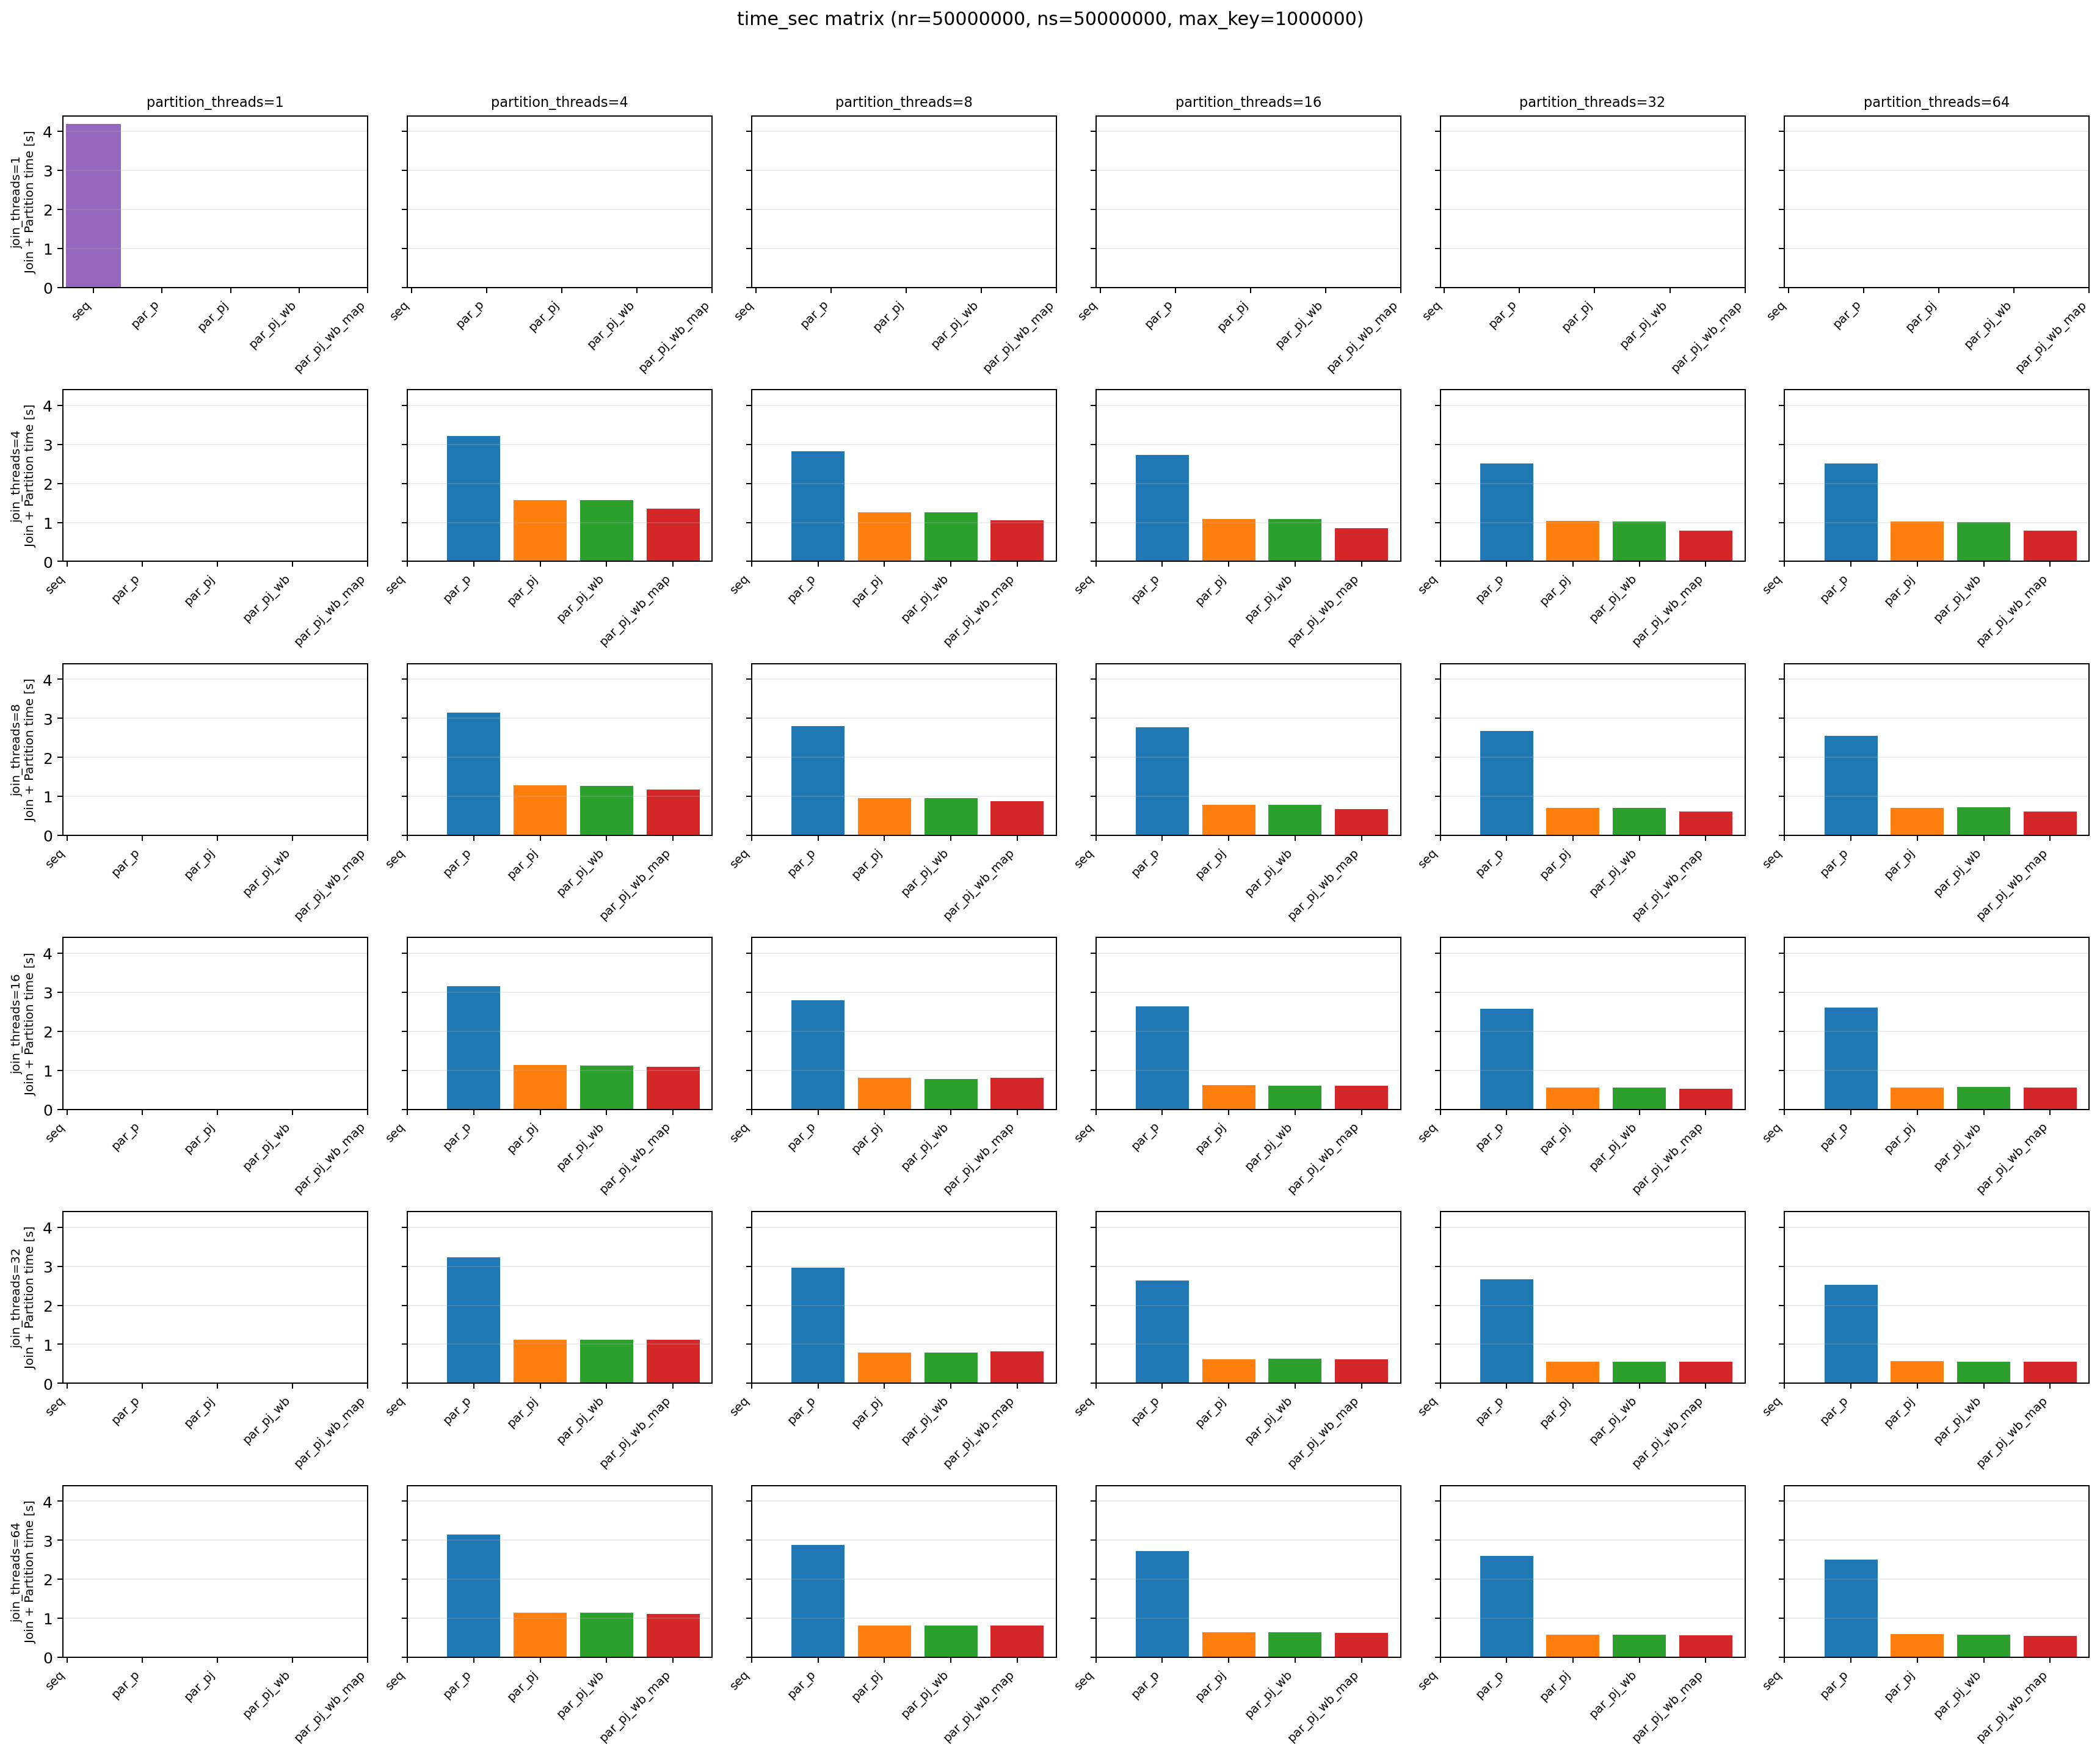
\includegraphics[width=0.62\linewidth]{../img/005_time_sec_matrix_nr50000000_ns50000000_maxkey1000000.png}
    \caption{Total execution-time (\texttt{time\_sec}) matrix for \(nr=ns=50\)M, \(P=256\), \(max\_key=10^6\).}
    \label{fig:time-sec-matrix}
\end{figure}

\begin{figure}[H]
    \centering
    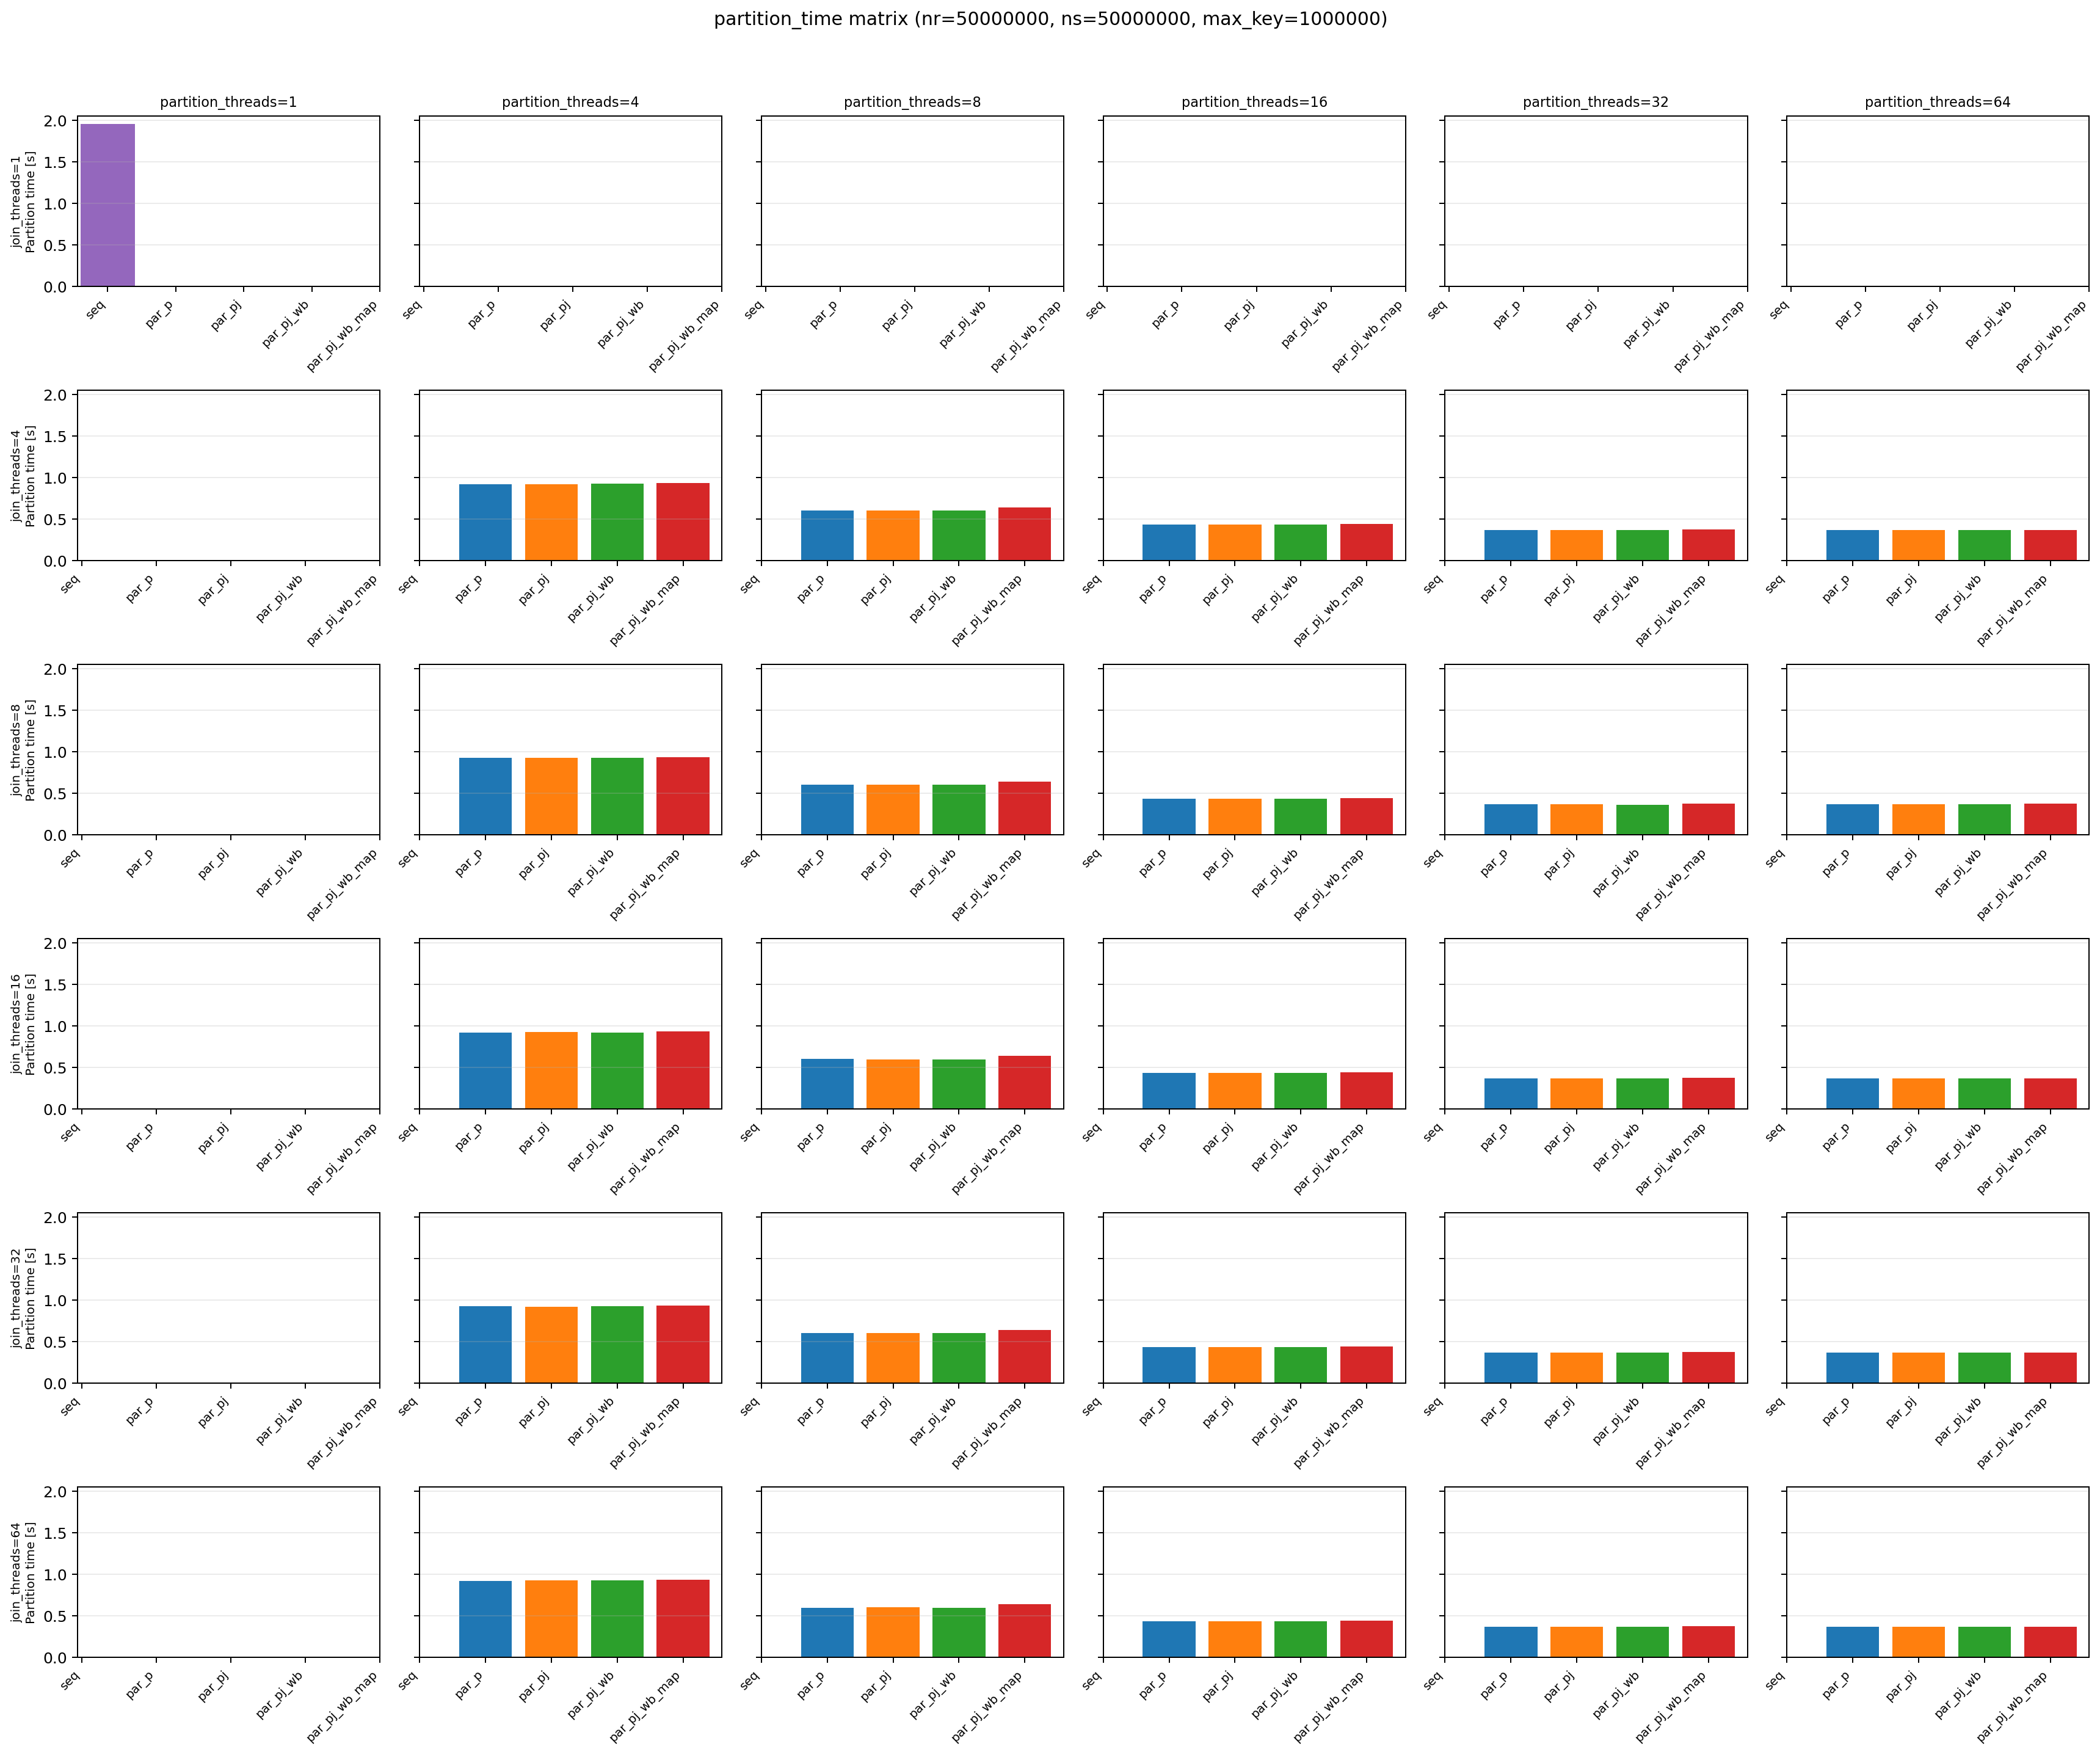
\includegraphics[width=0.49\linewidth]{../img/001_partition_time_matrix_nr50000000_ns50000000_maxkey1000000.png}\hfill
    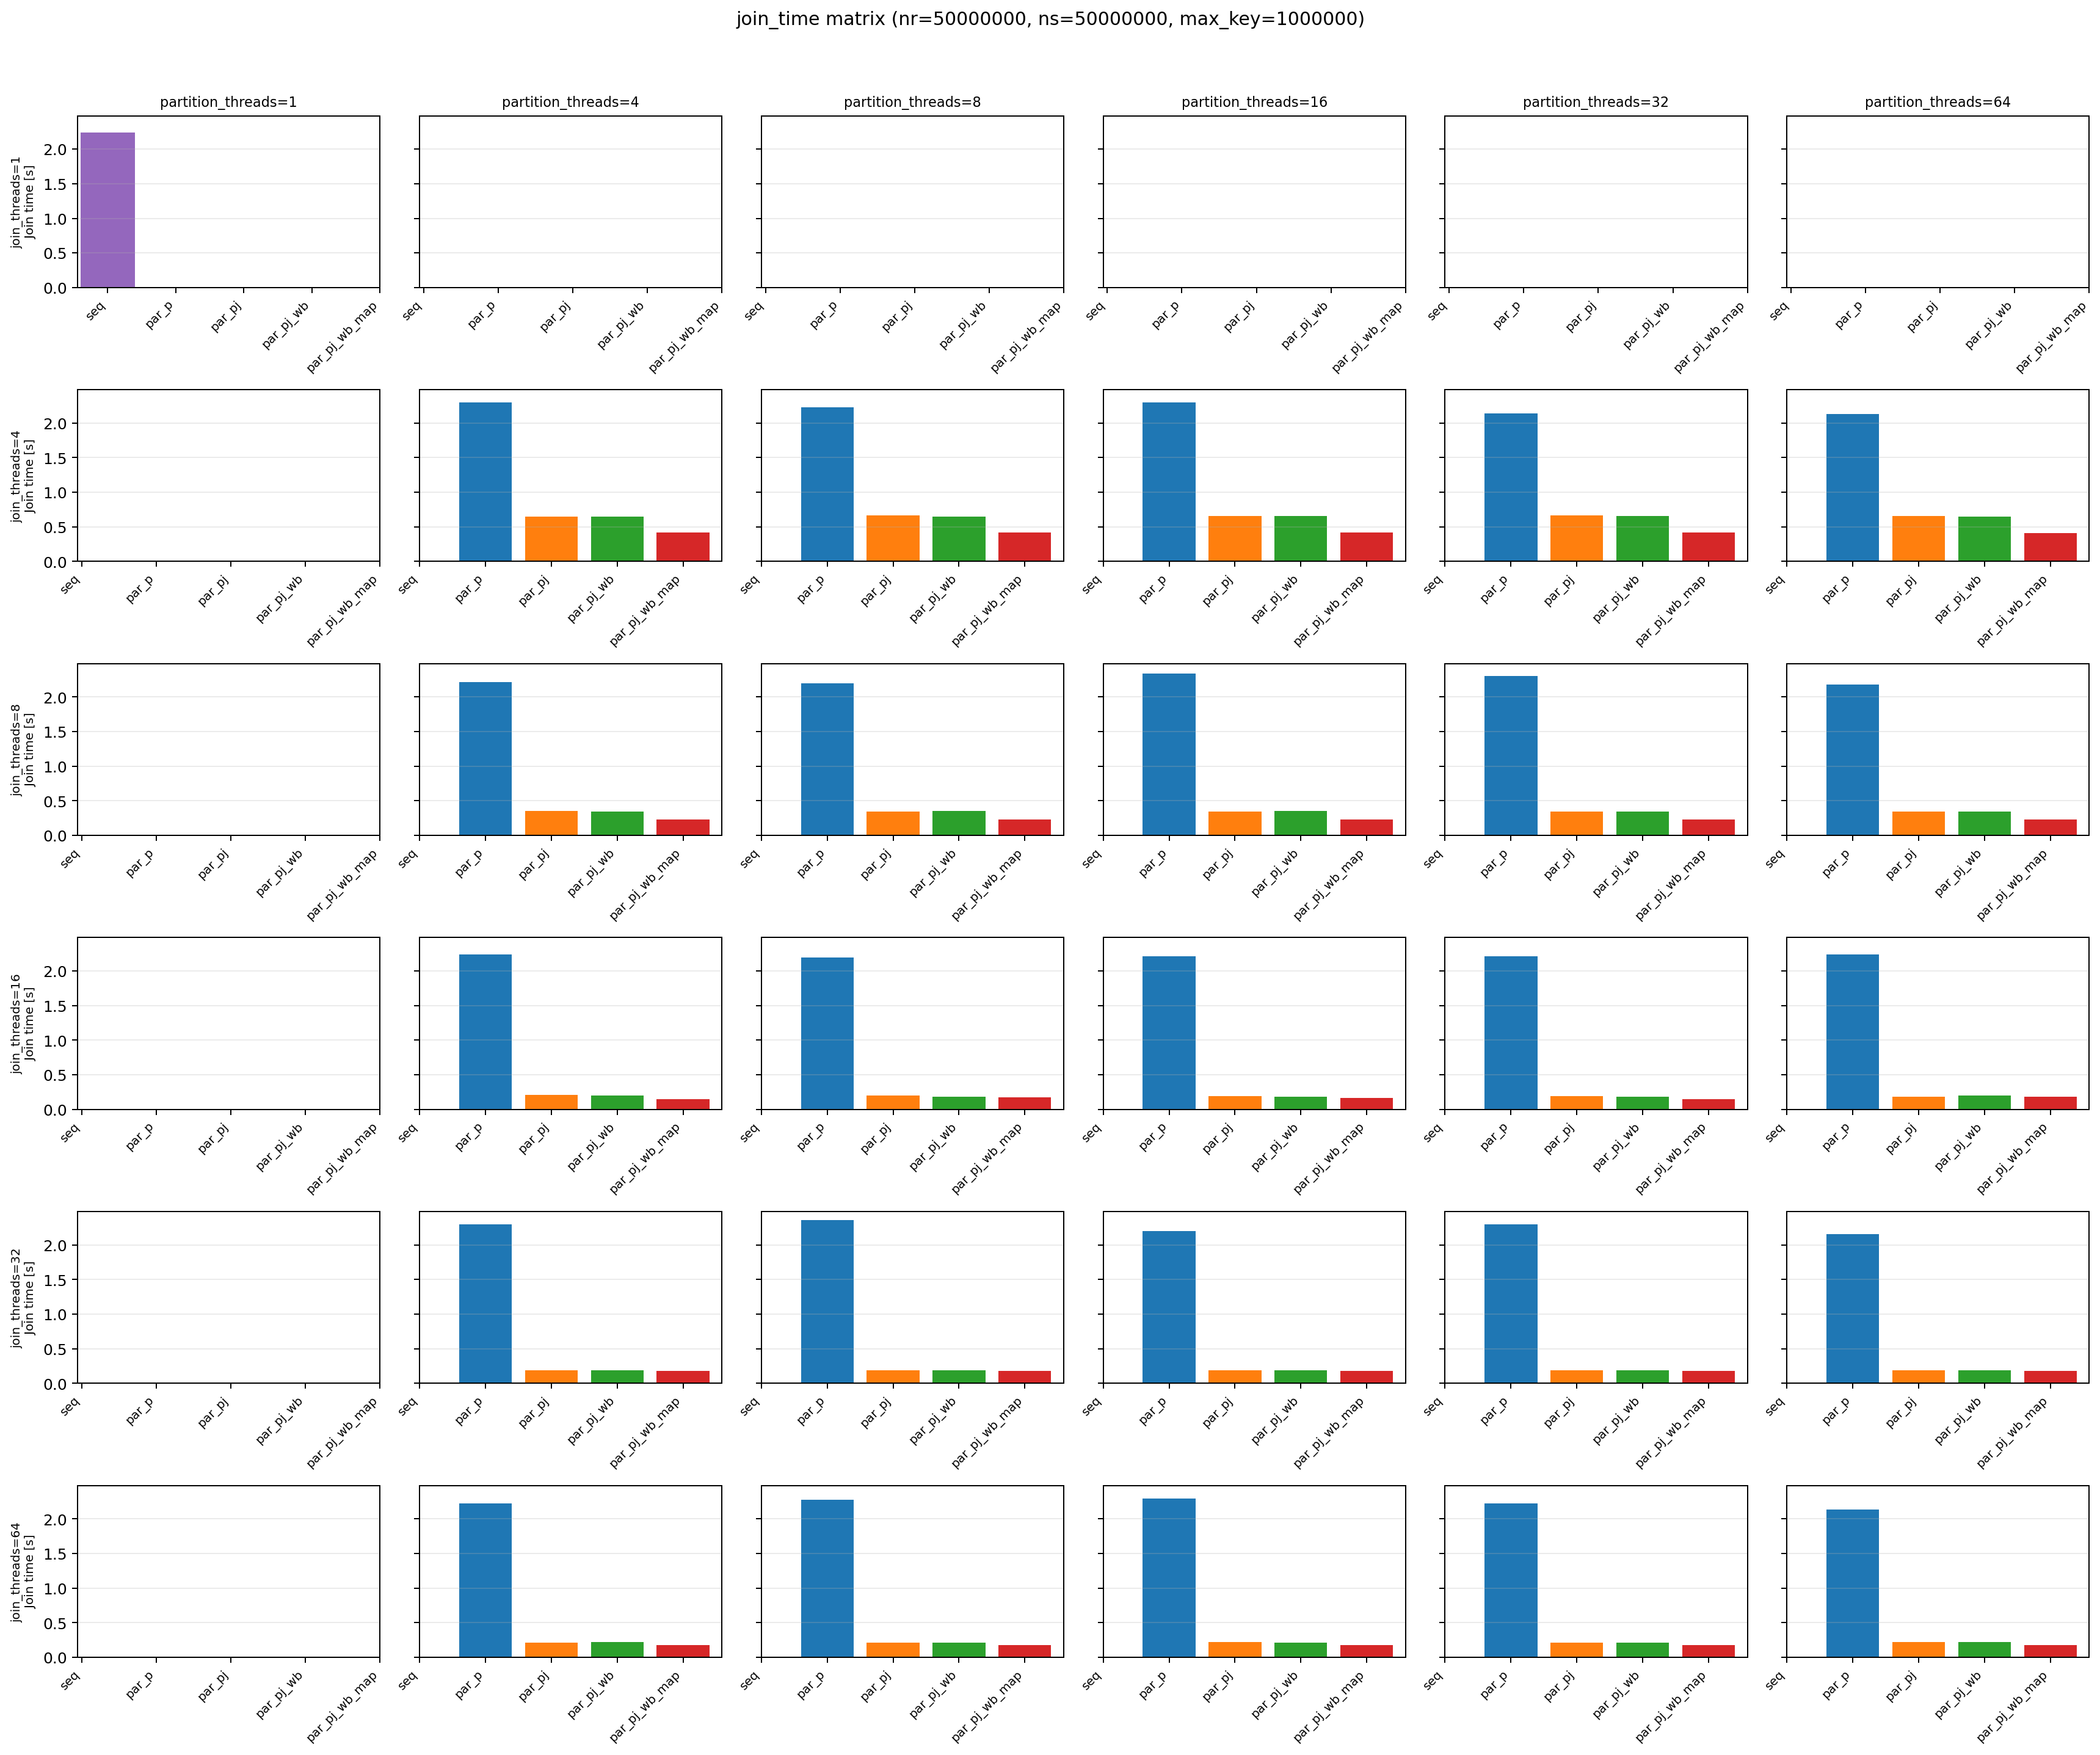
\includegraphics[width=0.49\linewidth]{../img/003_join_time_matrix_nr50000000_ns50000000_maxkey1000000.png}
    \caption{Partition-time and join-time matrices for \(nr=ns=50\)M, \(P=256\), \(max\_key=10^6\).}
    \label{fig:times-matrices}
\end{figure}

Partition time scales well from 4 to 32 threads, then flattens:
\begin{itemize}
    \item around \(0.92\) s at 4 partition threads;
    \item around \(0.36\)--\(0.37\) s at 32--64 partition threads.
\end{itemize}
This indicates good early scaling followed by memory-system saturation.

Join time is where variants differ the most. The executables \texttt{par\_pj} and \texttt{par\_pj\_wb} reduce join time to about \(0.18\) s in the best area.  
The \texttt{par\_pj\_wb\_map} variant improves further, reaching \(0.13\) s (best run, 32 partition threads and 16 join threads), confirming that data-structure locality in build/probe is a major factor.

\subsection{Strong Scaling}
Strong scaling is measured by fixing input size and increasing threads.
\begin{figure}[H]
    \centering
    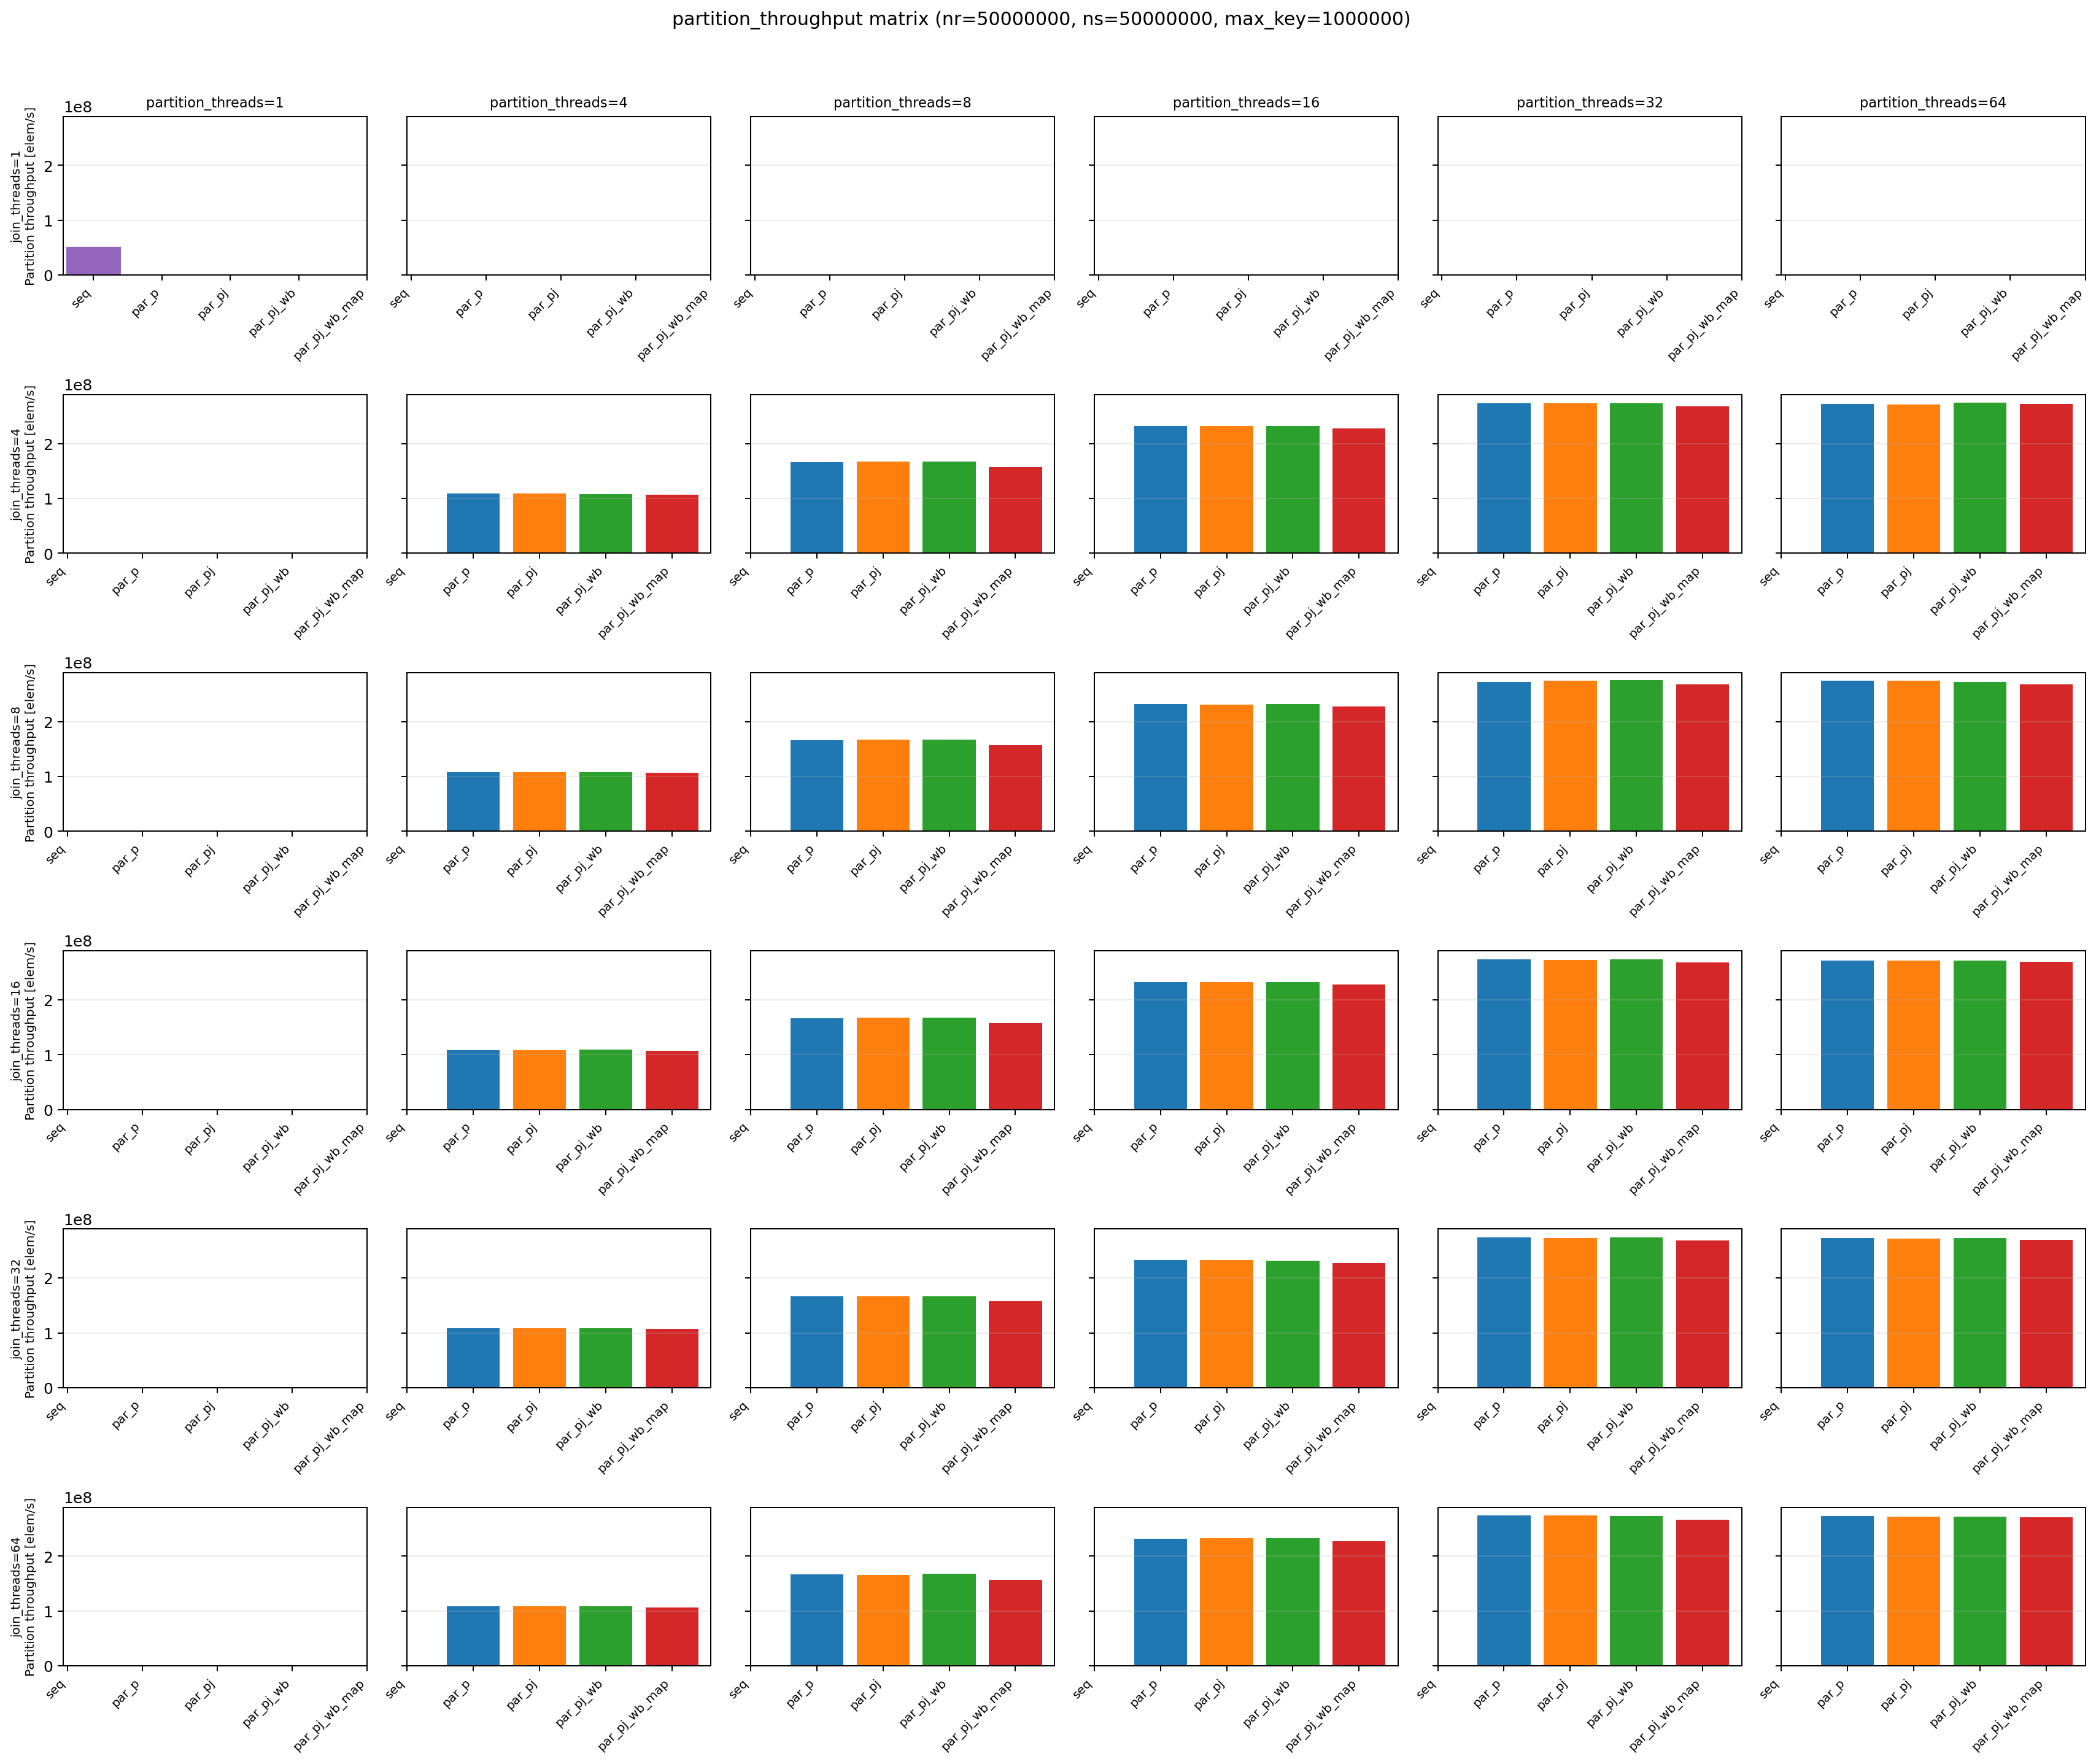
\includegraphics[width=0.49\linewidth]{../img/007_partition_throughput_matrix_nr50000000_ns50000000_maxkey1000000.png}\hfill
    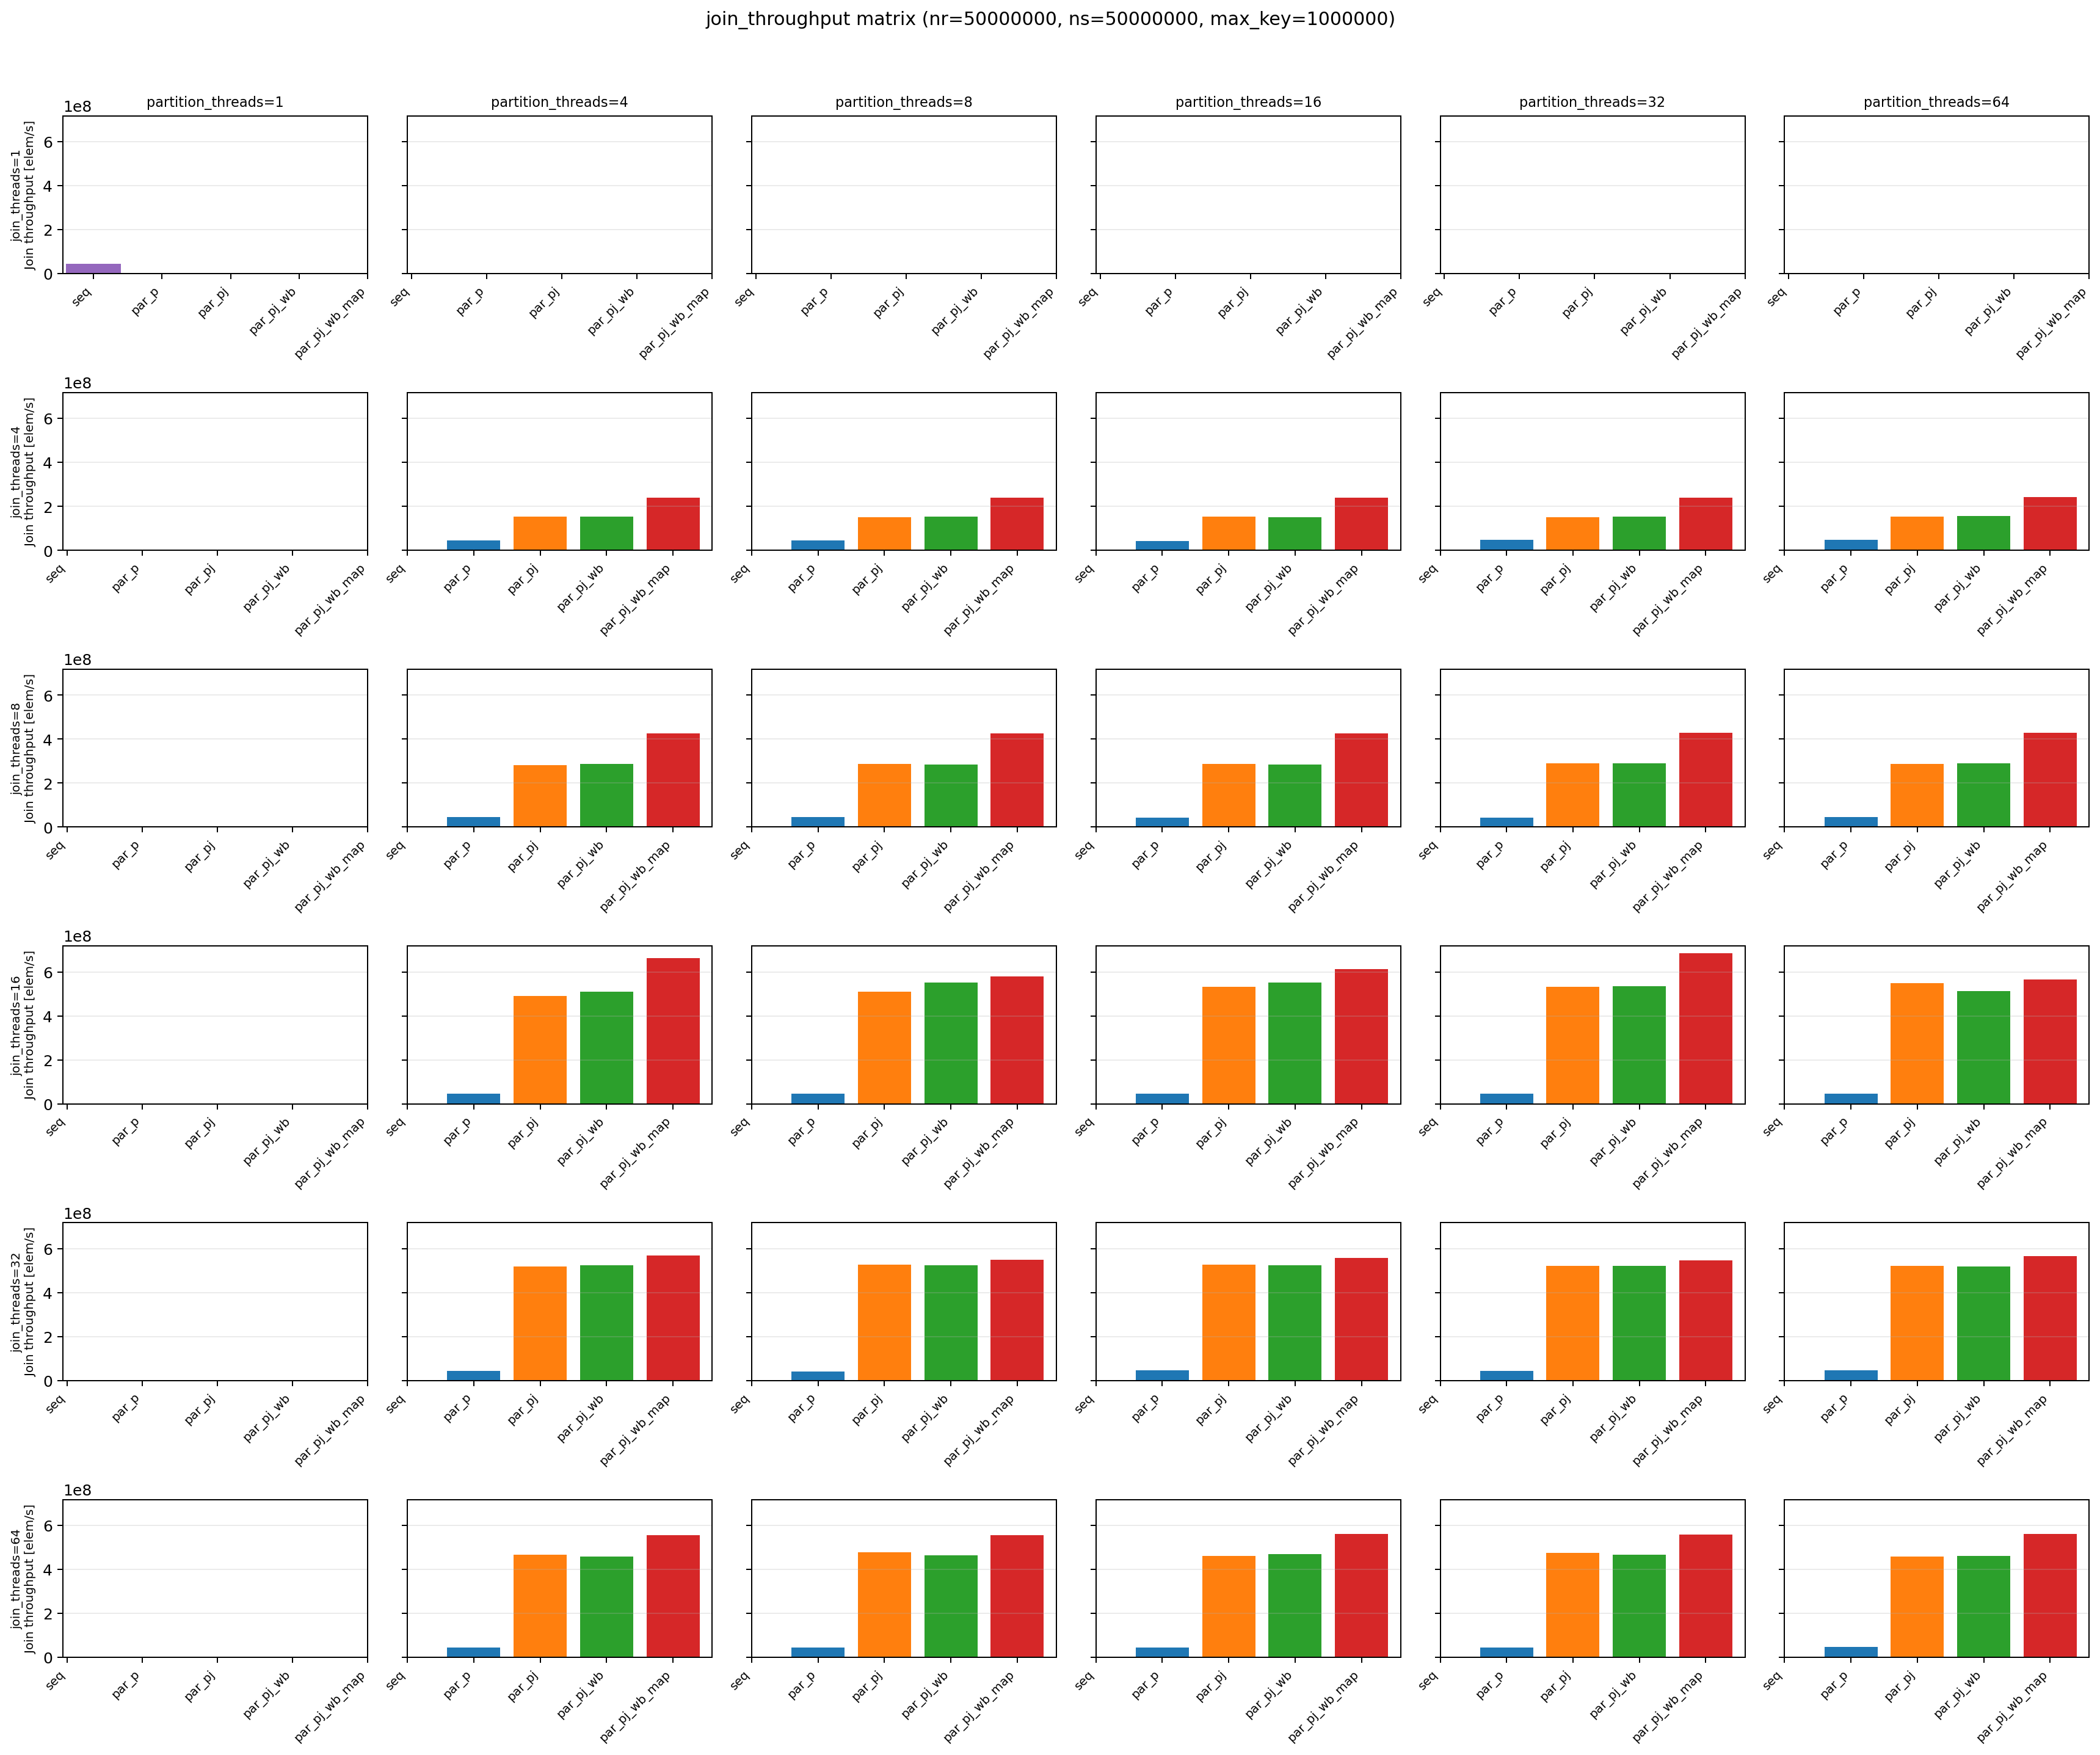
\includegraphics[width=0.49\linewidth]{../img/008_join_throughput_matrix_nr50000000_ns50000000_maxkey1000000.png}
    \caption{Partition-throughput and join-throughput matrices under fixed problem size.}
    \label{fig:strong-phase}
\end{figure}

\begin{wrapfigure}[10]{r}{0.42\textwidth}
    \hspace{1.0em}
    \vspace{-0.4em}
    \centering
    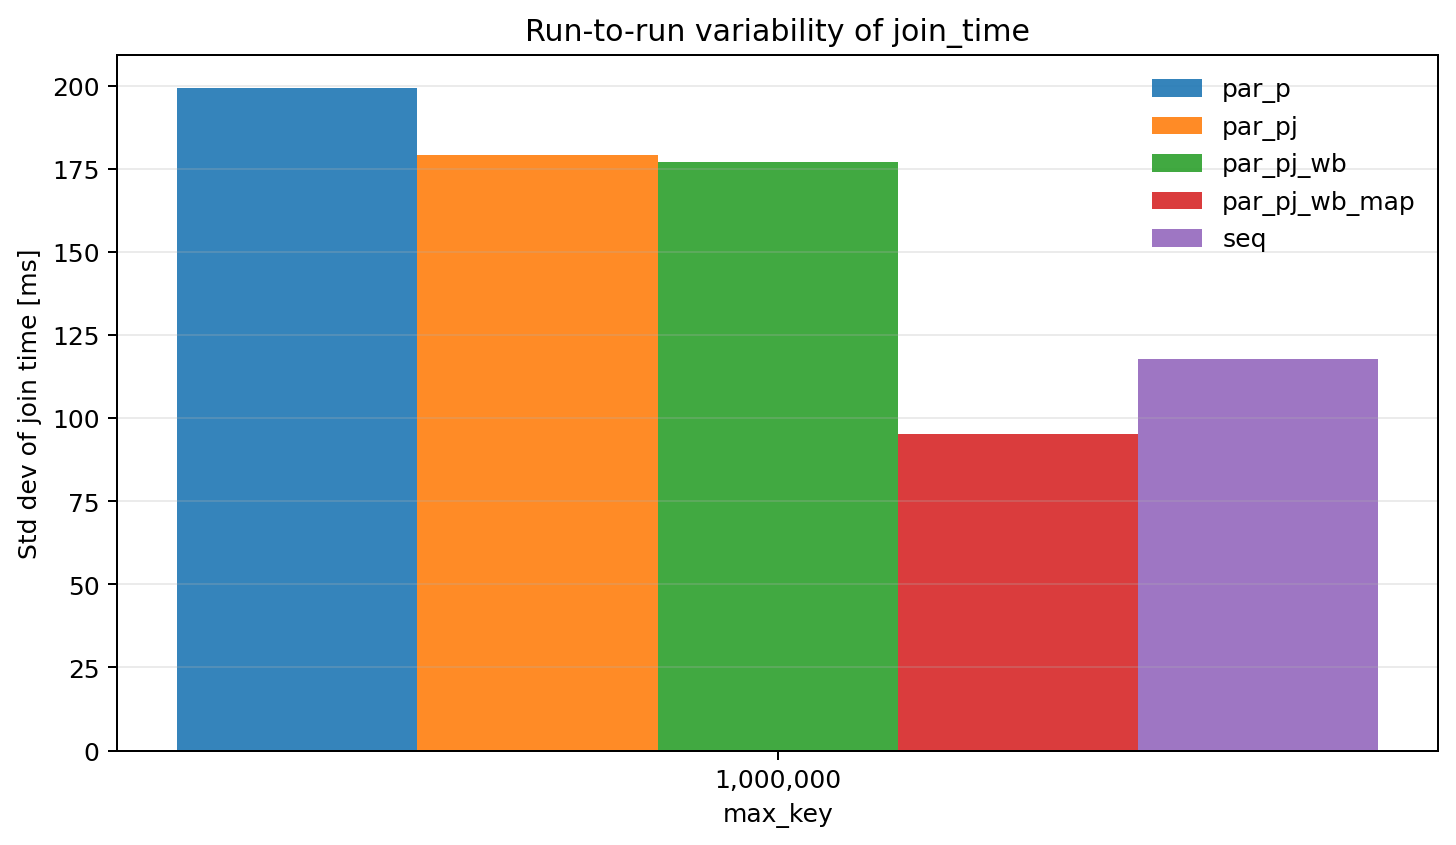
\includegraphics[width=\linewidth]{../img/004_std_join_time_by_max_key.png}
    \caption{Standard deviation of \texttt{join\_time}.}
    \label{fig:std-join-wrap}
    \vspace{-0.8em}
\end{wrapfigure}

On the diagonal (\(T_{part}=T_{join}\)), \texttt{par\_pj\_wb\_map} reaches:

\begin{itemize}
    \item speedup \(3.09\times\) at 4 threads;
    \item speedup \(6.87\times\) at 16 threads;
    \item speedup \(7.62\times\) at 64 threads.
\end{itemize}

Scaling is strong up to about 32 threads, then gains are smaller. This is coherent with the partition plateau and with increased overhead/imbalance sensitivity in the join stage at high thread counts.

In fact, the best result is got with \texttt{par\_pj\_wb\_map} using 16 join threads and 32 partition threads, with a speedup of about \(8.26\times\).

\subsection{Weak Scaling}
Weak-scaling results are now measured with a dedicated campaign (\texttt{weak\_scaling.cpp}) and grid:
\(N \in \{10,20,40,80\}\) million records per relation, \(T \in \{4,8,16,32\}\), and \(T_{part}=T_{join}\), with \(P=256\), seed \(=13\), and \(max\_key=10^6\).  
Each \((N,T)\) point is repeated 5 times, then averaged.

The weak-scaling curves are consistent across input sizes. Relative to 4 threads (same \(N\)):
\begin{itemize}
    \item at 8 threads, speedup is about \(1.65\times\);
    \item at 16 threads, speedup is about \(2.36\)--\(2.55\times\);
    \item at 32 threads, speedup is about \(2.64\)--\(2.82\times\).
\end{itemize}
The best observed weak-scaling speedup is \(2.82\times\) (for \(N=80\)M at 32 threads). This indicates good scalability trend with non-ideal efficiency at high thread counts, consistent with memory traffic and synchronization overheads.

\begin{figure}[H]
    \centering
    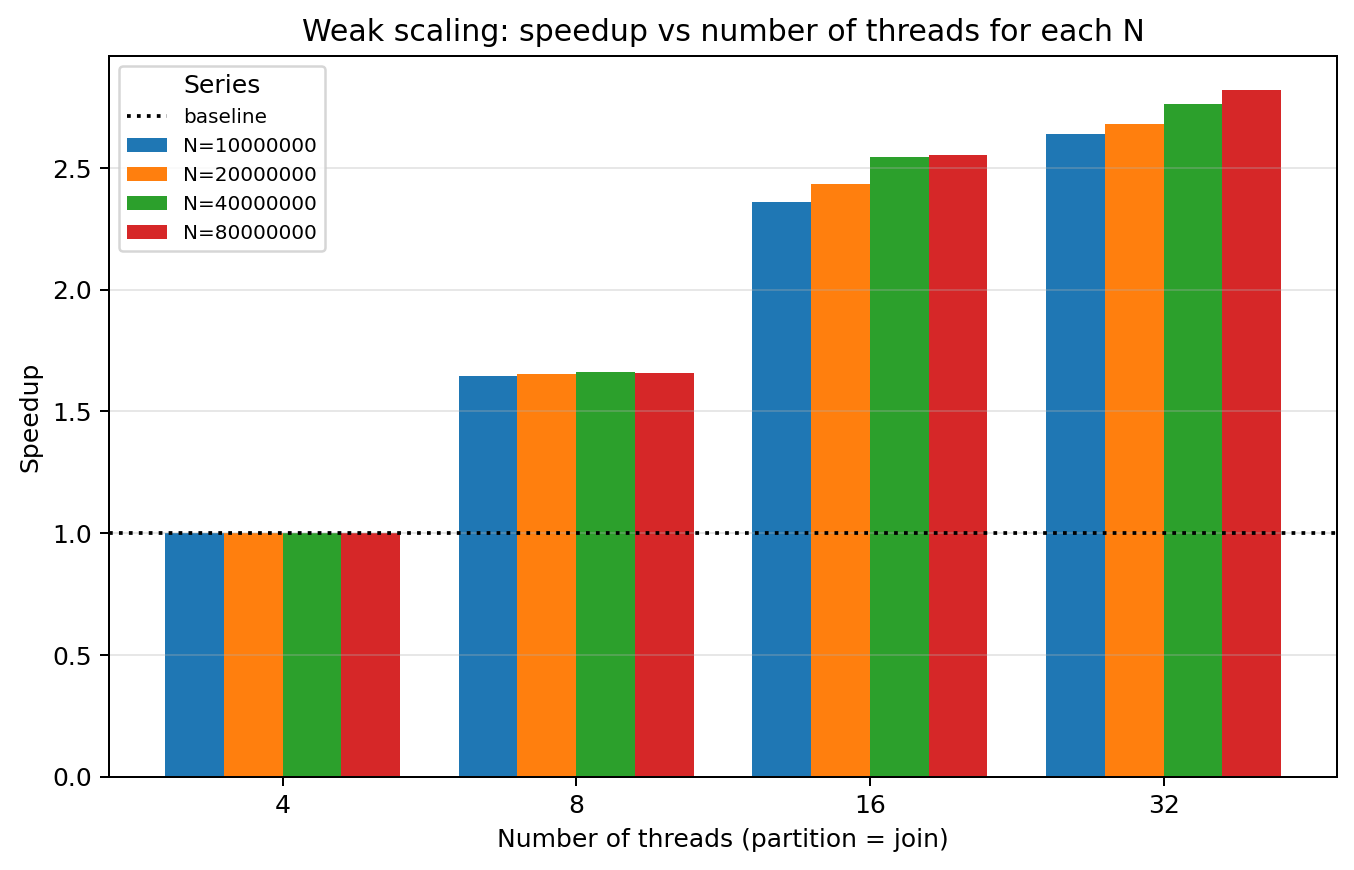
\includegraphics[width=0.68\linewidth]{../img/010_weak_scaling_speedup_vs_threads_by_N_weak_scaling.png}
    \caption{Weak-scaling speedup versus number of threads for each \(N\).}
    \label{fig:weak-scaling}
\end{figure}

\subsection{Speedup}
Global speedup is computed against the sequential mean total time (\(4.191\) s).
\begin{figure}[H]
    \centering
    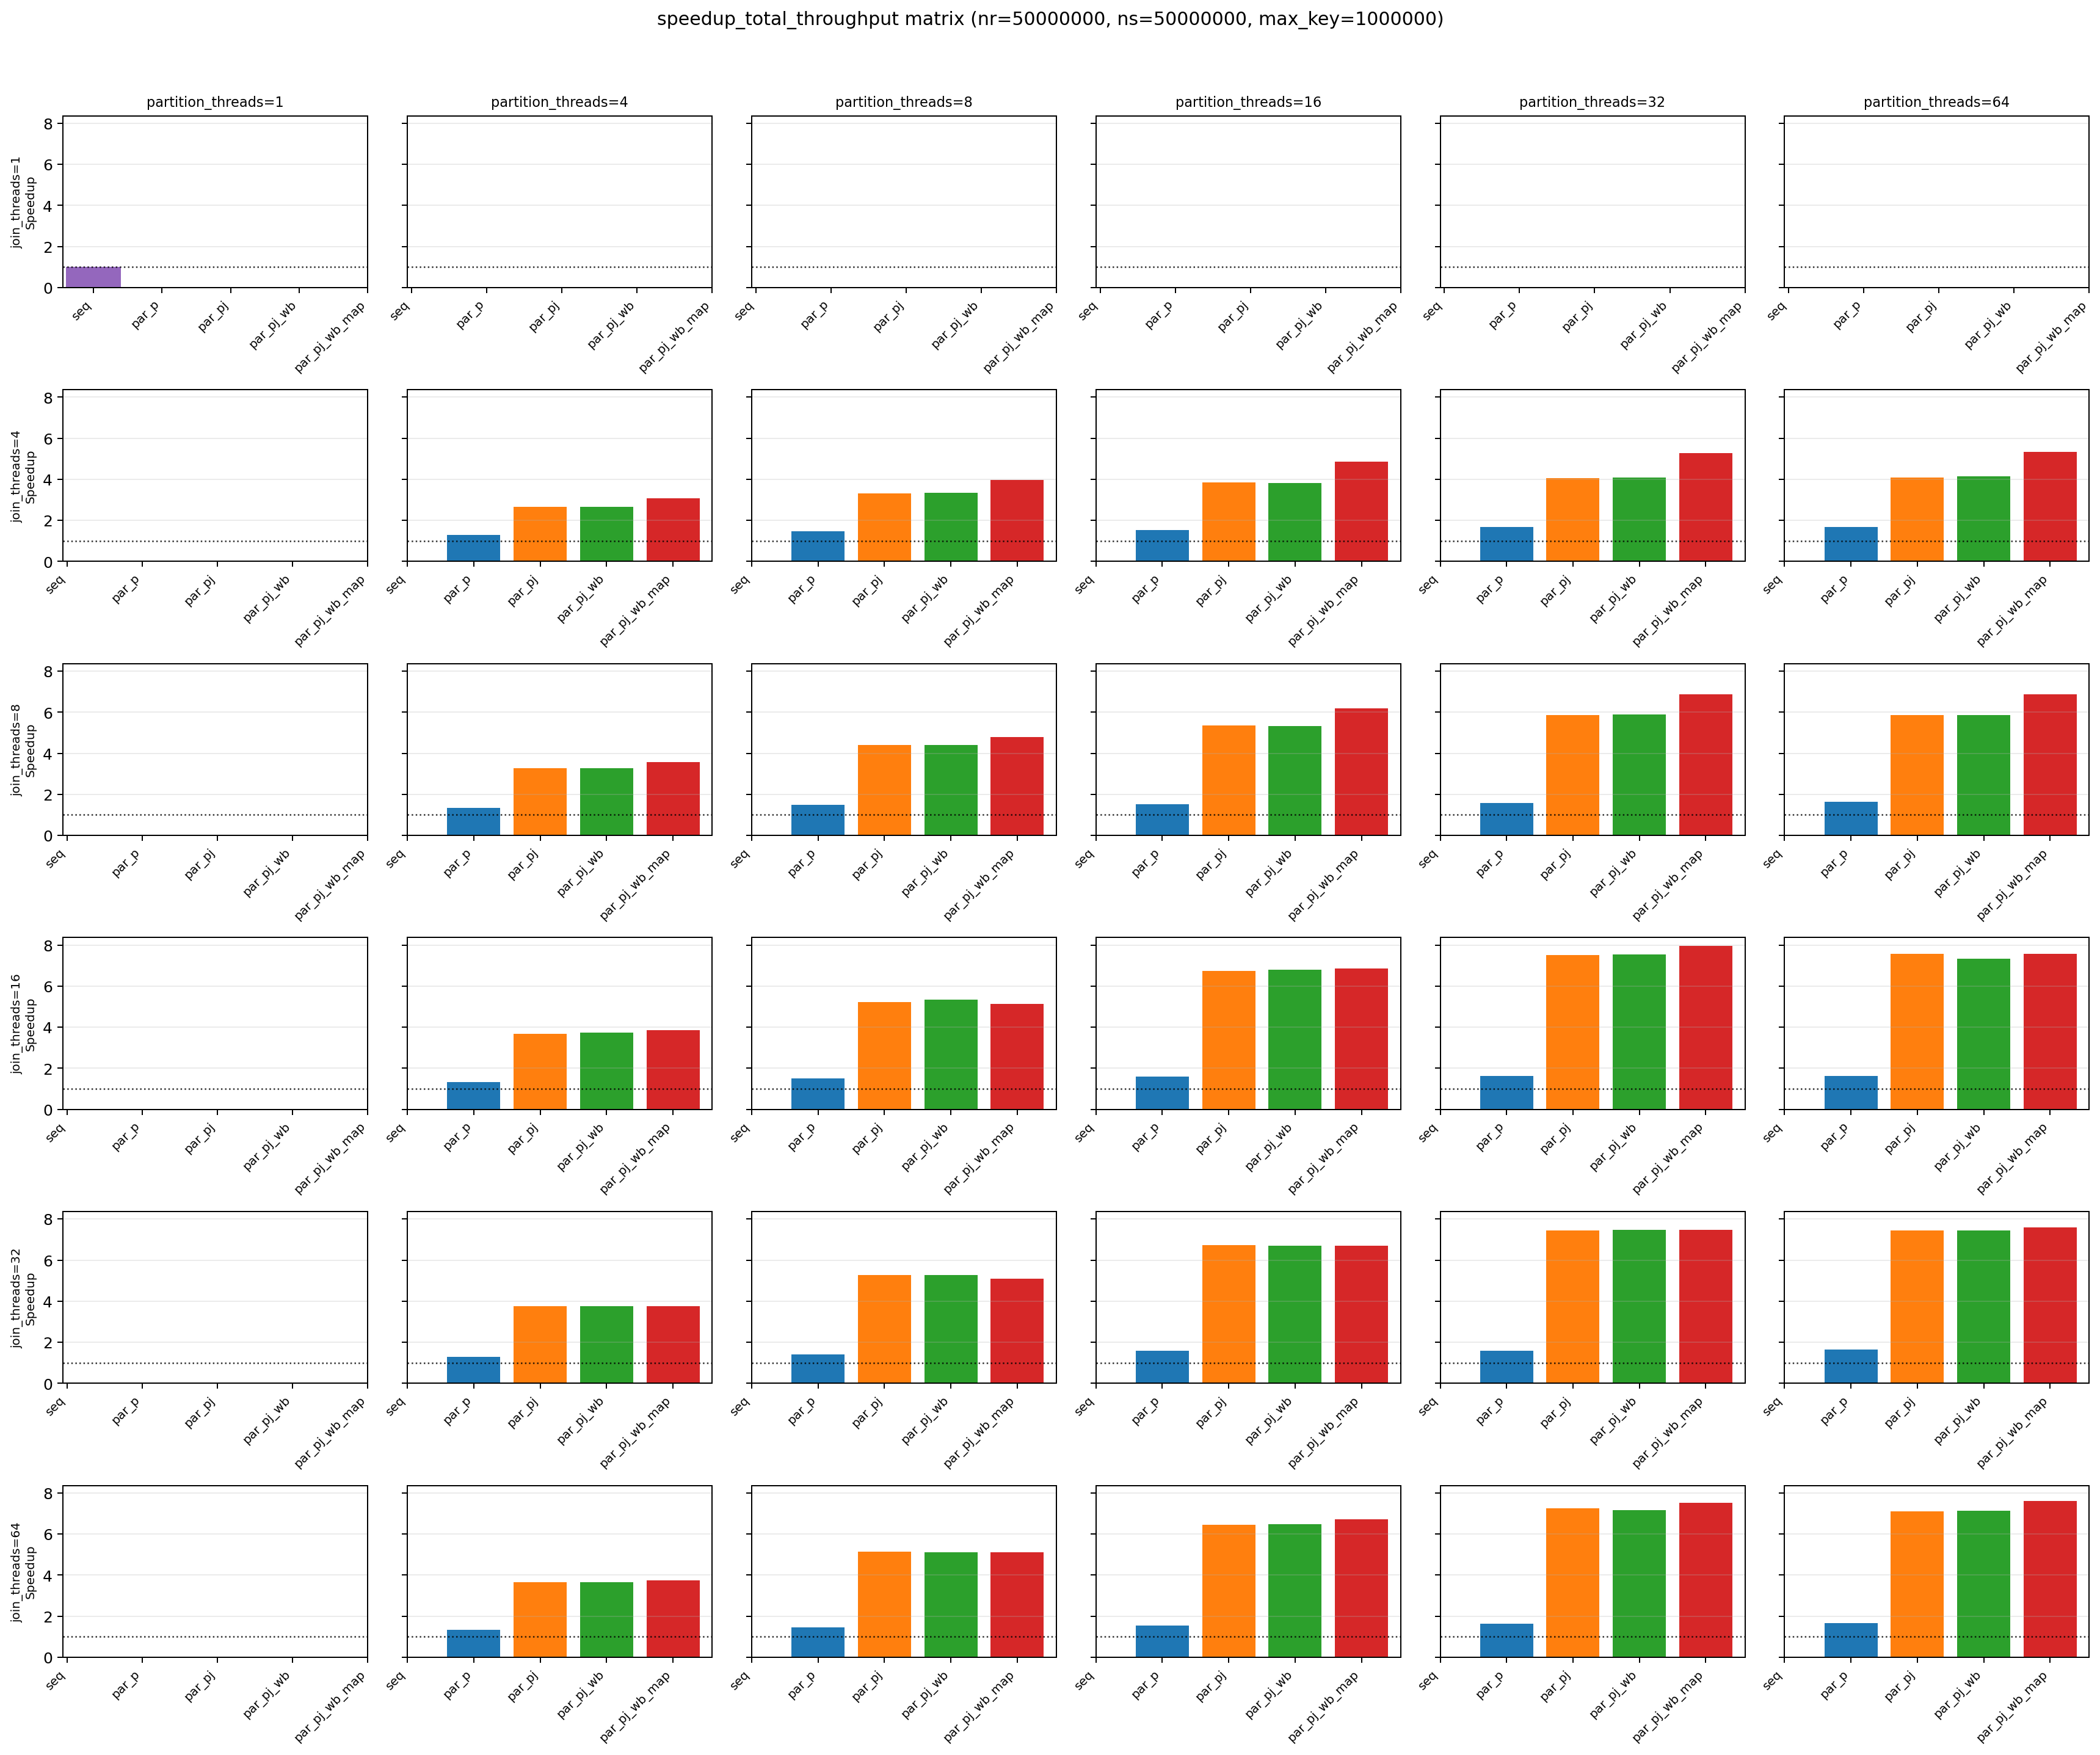
\includegraphics[width=0.62\linewidth]{../img/006_speedup_total_throughput_matrix_nr50000000_ns50000000_maxkey1000000.png}
    \caption{Total speedup matrix over thread combinations and variants.}
    \label{fig:speedup}
\end{figure}

\begin{table}[H]
    \centering
    \begin{tabular}{lrrrr}
        \toprule
        Variant & Best \(T_{part}\) & Best \(T_{join}\) & Best time [s] & Speedup \\
        \midrule
        \texttt{hashjoin\_par\_p} & 64 & 32 & 2.394 & \(1.75\times\) \\
        \texttt{hashjoin\_par\_pj} & 64 & 16 & 0.549 & \(7.63\times\) \\
        \texttt{hashjoin\_par\_pj\_wb} & 32 & 16 & 0.545 & \(7.69\times\) \\
        \texttt{hashjoin\_par\_pj\_wb\_map} & 32 & 16 & 0.507 & \(8.26\times\) \\
        \bottomrule
    \end{tabular}
    \caption{Best observed configuration per executable (baseline: sequential mean total time).}
    \label{tab:best-speedups}
\end{table}

The table confirms the optimization trajectory: partition-only parallelization gives limited gains, while parallel join plus balanced scheduling gives the main jump; flatter data structures in \texttt{par\_pj\_wb\_map} provide the final improvement.

\section{Conclusions}
The results show a clear progression:
\begin{itemize}
    \item parallelizing only partitioning is not sufficient (speedup capped around \(1.75\times\));
    \item parallelizing join is the dominant improvement (around \(7.6\times\));
    \item workload balancing improves robustness of high-thread runs;
    \item locality-oriented structures (\texttt{par\_pj\_wb\_map}) deliver the best result (\(8.26\times\)).
\end{itemize}

So, for this workload, the main insights are that join-phase optimization dominates total performance, while partition scaling saturates earlier and sets a practical upper bound unless data movement costs are further reduced. The added weak-scaling campaign confirms the same trend on increasing problem sizes, with diminishing efficiency at high thread counts.

\end{document}
